\documentclass[tikz]{standalone}

\usetikzlibrary{arrows}

\begin{document}

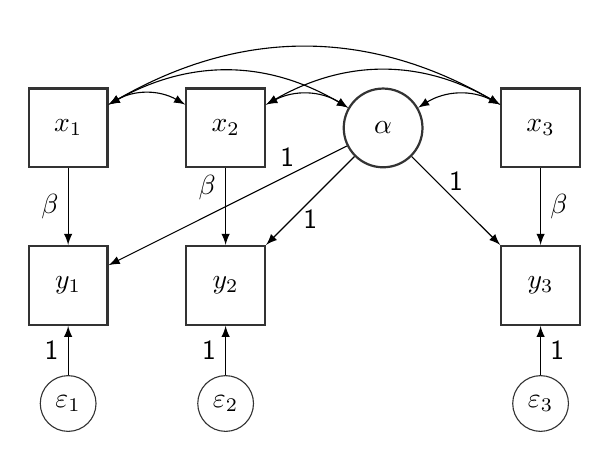
\begin{tikzpicture}
% Node styles ---
\tikzstyle{man} = [rectangle, thick, minimum size = 1cm, draw = black!80, fill = white!100, font = \sffamily] % Manifest variables
\tikzstyle{lat} = [circle, thick, minimum size = 1cm, draw = black!80, fill = white!100, font = \sffamily] % Latent variables
\tikzstyle{err} = [circle, draw = black!80, fill = white!100, font = \sffamily] % Errors 
% Edge styles
\tikzstyle{con} = [-latex, font = \sffamily] % Effects
\tikzstyle{cons} = [-latex, font = \sffamily\small] % Effects with smaller font 
\tikzstyle{cor} = [latex-latex, font = \sffamily] % Correlations
% Begin Figure ---
% Nodes 
\node at (+0.0,+0.0) [man] (x1) {$x_{1}$};
\node at (+2.0,+0.0) [man] (x2) {$x_{2}$};
\node at (+6.0,+0.0) [man] (x3) {$x_{3}$};
\node at (+4.0,+0.0) [lat] (eta) {$\alpha$};
\node at (+0.0,-2.0) [man] (y1) {$y_{1}$};
\node at (+2.0,-2.0) [man] (y2) {$y_{2}$};
\node at (+6.0,-2.0) [man] (y3) {$y_{3}$};
\node at (+0.0,-3.5) [err] (e1) {$\varepsilon_{1}$};
\node at (+2.0,-3.5) [err] (e2) {$\varepsilon_{2}$};
\node at (+6.0,-3.5) [err] (e3) {$\varepsilon_{3}$};
% Paths
\path (x1) edge [con, draw = black!100, left] node {$\beta$} (y1);
\path (x2) edge [con, draw = black!100, left, near start] node {$\beta$} (y2);
\path (x3) edge [con, draw = black!100, right] node {$\beta$} (y3);
\path (e1) edge [con, draw = black!100, left] node {1} (y1);
\path (e2) edge [con, draw = black!100, left] node {1} (y2);
\path (e3) edge [con, draw = black!100, right] node {1} (y3);
\path (eta) edge [con, draw = black!100, above, near start] node {1} (y1);
\path (eta) edge [con, draw = black!100, below] node {1} (y2);
\path (eta) edge [con, draw = black!100, above] node {1} (y3);
% correlations
\path (x1) edge [cor, bend left] node {} (x2);
\path (x1) edge [cor, bend left] node {} (eta);
\path (x1) edge [cor, bend left] node {} (x3);
\path (x2) edge [cor, bend left] node {} (eta);
\path (x2) edge [cor, bend left] node {} (x3);
\path (x3) edge [cor, bend right] node {} (eta);
\end{tikzpicture}

\end{document}